Ein RC-Schwingkreis besteht in der Regel aus einem Kondensator mit der
Kapazität $C$ und diner Spule, die eine Induktivität $L$ liefert.
Diese beiden Bauteile dienen hier als Energiespeicher.
In einem idealen Schwingkreis wird eine einmal eingespeicherte Energie
immer zwischen beiden genannten Elementen ausgetauscht.
Dieser Austausch kommt durch die Entladung des Kondensators zustande, bei welcher
in der Spule ein Magnetfeld aufgebaut wird. Wird dieses Magnetfeld abgebaut,
lädt sich der Kondensator auf und der Vorgang beginnt von neuem.
Wird ein gedämpfter, also ein realer Schwingkreis, betrachtet, ist neben der
Spule und dem Kondensator noch ein ohmscher Widerstand $R$ vorhanden.
Über diesen wird die Energie in Wärme umgewandelt und somit aus dem
Schwingkreis entfernt. $R$ ist demnach ein Dämpfungsfaktor.
Der schematische Aufbau eines $RCL$-Schwingkreises ist in Abbildung \ref{fig:rcl}
zu sehen.
\begin{figure}[H]
  \centering
  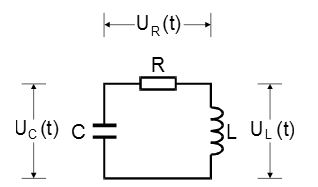
\includegraphics{Bilder/RCL.JPG}
  \caption{Schematischer Aufbau eines $RCL$-Kreises\cite{354}}
  \label{fig:rcl}
\end{figure}
Die Werte von $U_\su{R}, U_\su{C}$ und $U_\su{L}$ bezeichnen hierbei die Spannung
die über dem jeweiligen Bauteil abfällt. Gemäß des 2. Kirchhoffschen Gesetzes
gilt:
\begin{equation}
  U_\su{R}(t) + U_\su{C}(t) + U_\su{L}(t) = 0.
  \label{eqn:kirch}
\end{equation}
Um eine Differentialgleichung der 2. Ordnung zu erhalten, wird die Spannung
durch den Strom $I$ ausgedrückt. Somit erhält man:
\begin{align*}
  U_\su{R}(t) &= RI(t) \\
  U_\su{C}(t) &= \frac{Q(t)}{C} \text{mit} I = Q \\
  U_\su{L}(t) &= LI ,
\end{align*}
was zu der Differentialgleichung
\begin{equation}
  I(t) + \frac{R}{L}I(t) + \frac{1}{LC}I(t) = 0 .
\end{equation}
Mit dem entsprechendem Ansatz ergibt sich für die Gleichung
\begin{equation}
  I(t)=\exp{-2\pi\mu t}(A_1\exp{i2\pi\nu t} + A_2\exp{-2i\pi\nu t})
\end{equation}
